\section{Results}\label{sec:results}

\begin{figure*}[t]
\centering
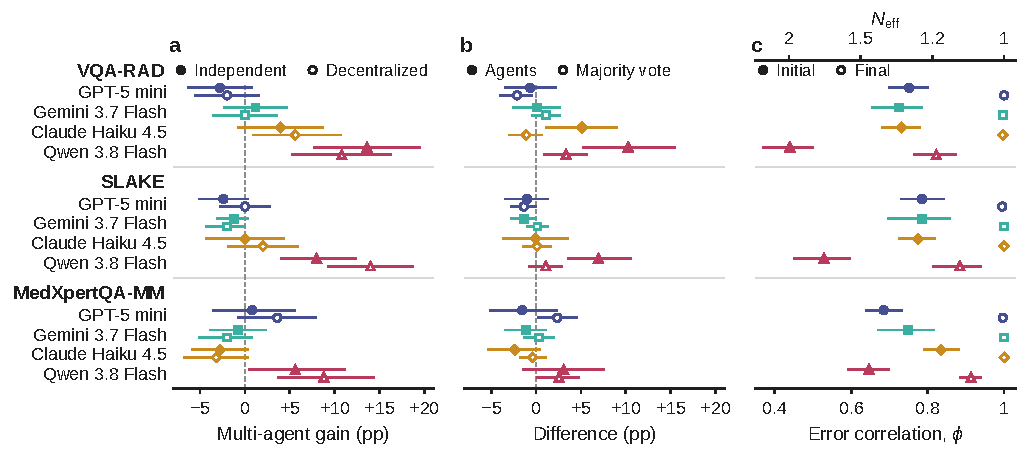
\includegraphics[width=\textwidth]{figures/fig3_panels.pdf}
\caption{\textbf{Nine agents from one VLM are worth fewer than two.}
Rows group models within data sets (250 items each).
(a) Multi-agent gain: Independent (filled) and Decentralized (open) accuracy minus single-agent accuracy.
(b) Independent gain decomposed into mean agent minus single-agent accuracy (Agents, filled) and majority minus mean agent accuracy (Majority vote, open).
(c) Error correlation $\phi$ for initial (filled) and final (open) answers; the top axis gives $N_{\mathrm{eff}}$.
Intervals are paired item-bootstrap 95\% CIs. Model colors as in \cref{fig:teaser}.}
\label{fig:panels}
\end{figure*}

\subsection{Nine agents are worth fewer than two}
Nine agents had an effective number of independent agents of $N_{\mathrm{eff}}=1.17$ to $1.99$ (\cref{fig:panels}).
For GPT-5 mini, Gemini 3.7 Flash, and Claude Haiku 4.5, the range was 1.17 to 1.39; Qwen 3.8 Flash reached 1.46 to 1.99.
The first three models' Independent multi-agent gains ranged from $-2.8$ to 4.0~pp, and their Decentralized gains from $-3.2$ to 5.6~pp.
Claude's Decentralized MAS gained 5.6~pp [0.8, 10.8] on VQA-RAD (Tabs.~S2--S5).

Qwen's larger gains arose mostly before majority voting: mean agent accuracy exceeded single-agent accuracy by 3.1 to 10.3~pp, while voting added 1.1 to 3.3~pp.
Its Independent MAS gained 13.6~pp [7.6, 19.6] on VQA-RAD, 8.0~pp [4.0, 12.4] on SLAKE, and 5.6~pp [0.4, 11.2] on MedXpertQA-MM.
Decentralized gains ranged from 8.8 to 14.0~pp.
For the other models, majority voting changed accuracy by $-2.1$ to 2.4~pp relative to mean agent accuracy (\cref{fig:panels}b).

Debate drove error correlation to 0.995 to 1.000 for GPT-5 mini, Gemini 3.7 Flash and Claude Haiku 4.5 and to 0.822 to 0.913 for Qwen 3.8 Flash (\cref{fig:panels}c).
Final answers were unanimous on 82.4\% to 100.0\% of items, but 8.9\% to 70.0\% of unanimous answers were wrong.

Mean agent accuracy and error correlation predicted majority accuracy with a mean residual of $-0.07$~pp across 108 systems on yes/no items.
The beta-binomial residual SD was 0.84~pp, and the largest absolute residual was 2.59~pp (\cref{fig:teaser,fig:supp-arithmetic}).
Across these systems, majority minus mean agent accuracy ranged from $-2.1$ to 5.6~pp over $\phi=0.44$ to $0.99$.

\begin{figure*}[t]
\centering
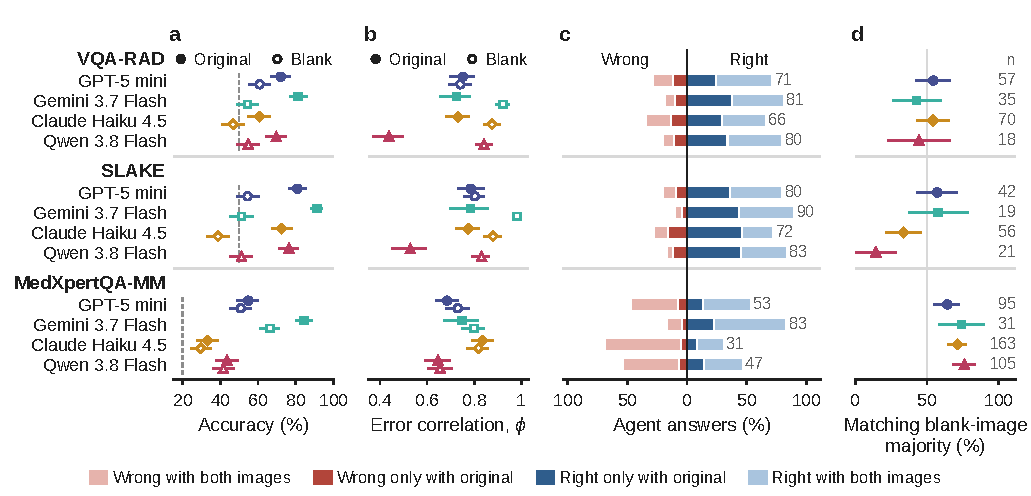
\includegraphics[width=\textwidth]{figures/fig4_prior.pdf}
\caption{\textbf{Most shared wrong answers on MedXpertQA-MM match the blank-image majority.}
(a) Single-agent accuracy with original (filled) and blank (open) images; dashed lines mark chance.
(b) Independent MAS error correlation with each image.
(c) Agent answers cross-tabulated by correctness: wrong with both images, wrong only with original, right only with original, and right with both images; end numbers give original-image accuracy.
(d) Shared wrong answers whose majority matches the blank-image majority; $n$ counts items with at least 7 of 9 agents wrong.
Each data set has 250 items. Intervals are item-bootstrap 95\% CIs. Model colors as in \cref{fig:teaser}.}
\label{fig:prior}
\end{figure*}

\subsection{Agents fall back on the language prior}
On MedXpertQA-MM, 64.2\% to 76.2\% of shared wrong answers matched the blank-image majority (\cref{fig:prior}d).
These items had at least 7 of 9 agents wrong with the original image.
The corresponding shares were 42.9\% to 54.4\% on VQA-RAD and 14.3\% to 57.9\% on SLAKE (Tabs.~S9--S10).

Replacing the image with a uniform gray blank image reduced single-agent accuracy by 11.2 to 26.8~pp on VQA-RAD and 25.2 to 40.0~pp on SLAKE (\cref{fig:prior}a).
On MedXpertQA-MM, losses were 4.0~pp [$-2.0$, 10.0] for GPT-5 mini, 3.6~pp [$-0.4$, 8.0] for Claude, and 2.0~pp [$-4.4$, 8.0] for Qwen.
Gemini lost 18.0~pp [12.0, 23.6] (Tabs.~S6--S8).

With blank images, Gemini, Claude, and Qwen had $\phi=0.841$ to $0.922$ on VQA-RAD and 0.831 to 0.982 on SLAKE (\cref{fig:prior}b).
Original-image ranges were 0.439--0.731 and 0.529--0.785, respectively.
Claude's blank-image correlation remained high after abstentions were excluded: 0.963 on VQA-RAD, 0.931 on SLAKE, and 0.852 on MedXpertQA-MM.
Reduced resolution changed $\phi$ in opposite directions across models: on VQA-RAD, GPT-5 mini fell from 0.752 to 0.644, while Qwen rose from 0.439 to 0.480 (\cref{fig:supp-resolution}).

On VQA-RAD, 24.1\% to 37.3\% of agent answers were correct only with the original image, versus 10.4\% to 13.6\% only with the blank image (\cref{fig:prior}c).
SLAKE shares were 36.3\% to 46.4\% versus 4.4\% to 15.8\%; MedXpertQA-MM shares were 8.1\% to 22.3\% versus 4.4\% to 7.9\%.
On MedXpertQA-MM, 12.3\% to 64.0\% were wrong with both images.

\begin{figure}[t]
\centering
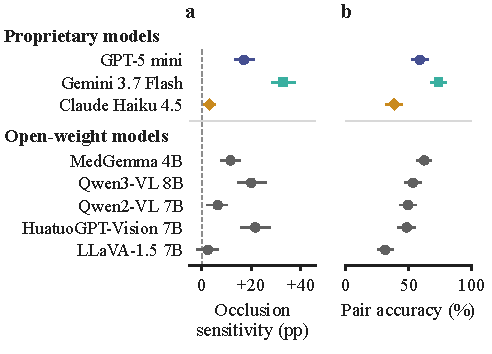
\includegraphics[width=\linewidth]{figures/fig5_region.pdf}
\caption{\textbf{Models differ in their sensitivity to the queried image region.}
(a) Occlusion sensitivity, target minus control answer-change rate, on SLAKE-target (250 items).
(b) Pair accuracy, both answers correct, on SLAKE-pairs (200 pairs with opposite reference answers).
Occlusion estimates average Independent MAS agents for proprietary models; pair accuracy uses single agents.
Open-weight models use one forward pass per item.
Intervals are item-bootstrap 95\% CIs; pairs are resampled intact in (b). Model colors as in \cref{fig:teaser}.}
\label{fig:region}
\end{figure}

\subsection{Models differ in where they look}
Gemini's occlusion sensitivity was 32.9~pp [28.2, 38.0], compared with 17.1~pp [13.2, 21.2] for GPT-5 mini and 3.2~pp [0.8, 5.7] for Claude (\cref{fig:region}a).
This difference subtracts answer changes under an equal-size control occlusion from those under target occlusion.
Open-weight estimates ranged from 2.4 to 21.6~pp; LLaVA-1.5 7B had 2.4~pp [$-2.0$, 6.8] (Tabs.~S11--S12).

Gemini also had the highest proprietary-model pair accuracy: 74.0\% [67.5, 80.0], versus 59.0\% for GPT-5 mini and 38.5\% for Claude (\cref{fig:region}b).
With the same question and opposite reference answers, agents changed their answer between images in 75.0\%, 62.0\%, and 42.5\% of pairs, respectively (Tabs.~S13--S14).
The remaining pairs received identical answers despite the change in reference answer.

\begin{figure*}[t]
\centering
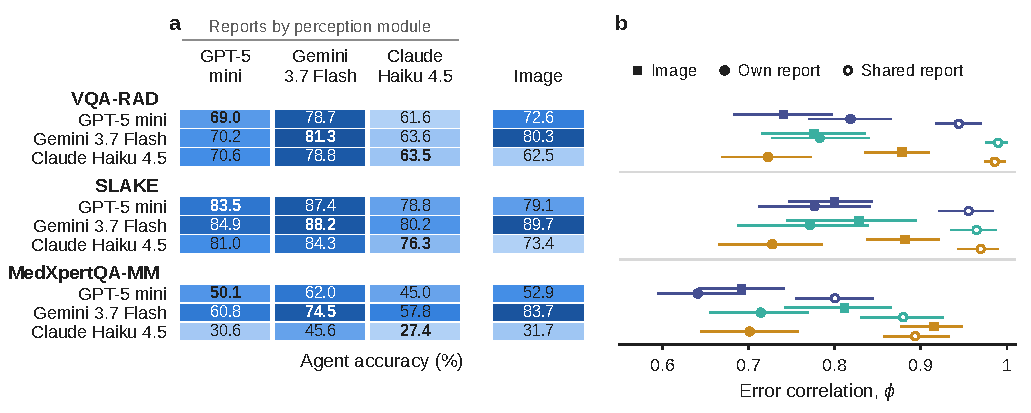
\includegraphics[width=\textwidth]{figures/fig6_report.pdf}
\caption{\textbf{Perception sets accuracy, while sharing a report increases error correlation.}
(a) Agent accuracy with its own query-agnostic report from the column's perception module, or with the image.
Rows identify reasoning modules within data sets (250 items each); shading scales within each data set.
Bold cells use the same model for both modules.
(b) Error correlation among 9 agents: image (filled square), own report (filled circle), and shared report (open circle), with same-model reports.
Intervals are item-bootstrap 95\% CIs. Model colors as in \cref{fig:teaser}.}
\label{fig:report}
\end{figure*}

\subsection{Perception sets accuracy; a shared report sets correlation}
Gemini's query-agnostic reports raised the other reasoning modules' accuracy by 6.1 to 16.3~pp over reading the image (\cref{fig:report}a).
The endpoint effects were 6.1~pp [1.4, 10.9] for GPT-5 mini and 16.3~pp [9.9, 22.6] for Claude on VQA-RAD.
Each agent read its own report without the image.
Across reasoning modules, Gemini reports yielded 78.7\% to 81.3\% accuracy on VQA-RAD and 84.3\% to 88.2\% on SLAKE.
Claude reports lowered the other reasoning modules' accuracy in 5 of 6 cells, by 7.9 to 25.9~pp.
The remaining cell, GPT-5 mini on SLAKE, differed by $-0.4$~pp [$-5.0$, 4.6] (Tabs.~S17--S19).

Under identical Gemini reports on MedXpertQA-MM, accuracy differed by reasoning module: Gemini achieved 74.5\%, GPT-5 mini 62.0\%, and Claude 45.6\%.
With GPT-5 mini reports, their accuracies were 60.8\%, 50.1\%, and 30.6\%, respectively.

The queried target was absent from 26.5\% to 30.8\% of SLAKE reports and from 25.8\% to 47.1\% of reports behind errors.
For Gemini reports, omissions occurred in 26.7\% overall and 33.6\% to 47.1\% of reports behind errors across reasoning modules.

Sharing one report raised $\phi$ to 0.800--0.990, compared with 0.641--0.818 when agents read their own reports from the same model (\cref{fig:report}b).
Both modules were held fixed in this comparison; only the report was shared.

\begin{figure}[t]
\centering
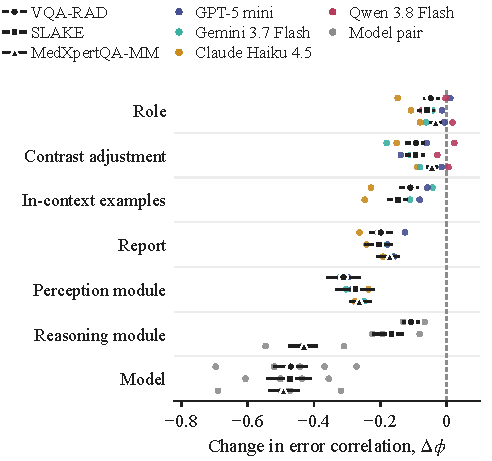
\includegraphics[width=\linewidth]{figures/fig7_contrasts.pdf}
\caption{\textbf{Changing the model reduces error correlation more than changing a component within one model.}
Matched $\Delta\phi$ compares agents differing in the named component with agents sharing it.
Black markers give data-set means: circle, VQA-RAD; square, SLAKE; triangle, MedXpertQA-MM (250 items each).
Colored dots give models; gray dots give model pairs.
In-context examples compare private with shared examples on VQA-RAD and SLAKE.
Report compares own with shared reports; reasoning-module contrasts hold the report fixed.
Intervals are item-bootstrap 95\% CIs. Model colors as in \cref{fig:teaser}.}
\label{fig:contrasts}
\end{figure}

\subsection{What makes two agents err together}
Changing the model produced the largest mean reduction in error correlation, 0.470 to 0.492 across data sets (\cref{fig:contrasts}).
Self-consistency samples of one model had $\phi=0.692$ to $0.915$ for the proprietary models and 0.442 to 0.629 for Qwen (Tabs.~S20--S22).
Mean reductions were 0.033--0.060 for role and 0.045--0.094 for contrast adjustment.
Private in-context examples reduced $\phi$ by 0.110--0.146 relative to shared examples; own reports reduced it by 0.172--0.204 relative to a shared report.
Changing the perception module reduced $\phi$ by 0.263--0.311.

The reasoning-module contrast was largest on MedXpertQA-MM: $\Delta\phi=-0.430$ [$-0.477$, $-0.389$], compared with $-0.263$ for the perception module.
Across data sets, reasoning-module contrasts ranged from $-0.430$ to $-0.108$ under identical reports.
Private examples also separated correlation from accuracy: for Claude on SLAKE, $\phi$ fell from 0.928 to 0.655 with private image examples, while MAS accuracy fell from 70.4\% to 68.8\% (Tabs.~S25--S28).
The additive regression is a secondary summary in Tabs.~S23--S24.

\begin{figure}[t]
\centering
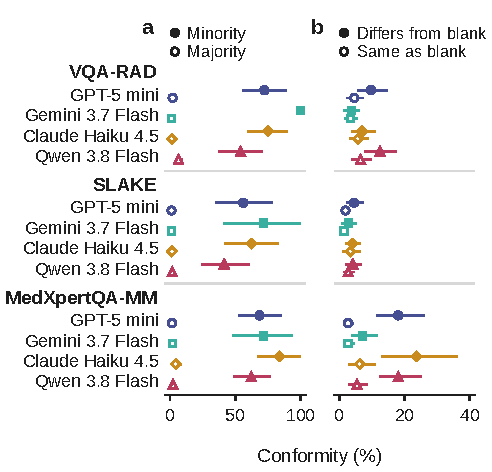
\includegraphics[width=\linewidth]{figures/fig8_discussion.pdf}
\caption{\textbf{Agents change correct minority answers to wrong answers during debate.}
Conformity is the share of initially correct agents whose final answer is wrong in the Decentralized MAS.
(a) Initial minority (filled) versus majority (open).
(b) Initial answer differs from (filled) or matches (open) the same agent's blank-image answer.
Rows group models within data sets (250 items each; 9 agents).
Intervals are item-bootstrap 95\% CIs. Model colors as in \cref{fig:teaser}.}
\label{fig:conformity}
\end{figure}

\subsection{Debate removes correct minority answers}
Agents changed 41.5\% to 100.0\% of correct initial minority answers to wrong answers during debate, versus 1.0\% to 6.5\% of correct majority answers (\cref{fig:conformity}a).
On MedXpertQA-MM, conformity was 7.2\% to 23.6\% when a correct initial answer differed from the same agent's blank-image answer, versus 2.6\% to 6.3\% when it matched (\cref{fig:conformity}b).
Paired differences ranged from 4.6~pp [0.8, 9.0] for Gemini to 17.4~pp [6.4, 29.7] for Claude (Tabs.~S15--S16).
Among correct answers that differed from the blank-image answer, 6.6\% to 23.5\% were initially in the minority on MedXpertQA-MM.

\subsection{Open-weight probes}
Blank images cost four of five open-weight models 16.4 to 19.2~pp on VQA-RAD; LLaVA-1.5 7B lost 2.0~pp (\cref{fig:supp-openweight}).
All five lost 16.0 to 48.8~pp on SLAKE.
On MedXpertQA-MM, original-image accuracy was 20.0\% to 24.4\%, versus 20.0\% to 23.6\% with blank images (Tabs.~S29--S30).
Mean visual reliance, the absolute change in log-odds of yes, ranged from 0.89 to 6.43 on VQA-RAD and 1.40 to 11.23 on SLAKE.
On MedXpertQA-MM, reliance measured by Kullback--Leibler divergence ranged from 0.10 to 0.88.

Error correlation between open-weight models ranged from 0.099 to 0.535 (Tab.~S31).
HuatuoGPT-Vision 7B and LLaVA-1.5 7B share the CLIP ViT-L/14-336 encoder.
Their correlation divided by its maximum given marginal error rates, $\phi/\phi_{\max}$, was 0.213 to 0.451; pairs with different encoders ranged from 0.148 to 0.725.
Proprietary-model shared wrong answers were associated with lower open-weight visual reliance on SLAKE: Spearman $\rho=-0.401$ [$-0.502$, $-0.295$].
It was $-0.048$ [$-0.165$, 0.068] on VQA-RAD and 0.006 [$-0.128$, 0.136] on MedXpertQA-MM.
